\chapter{Methodology}
\label{sec:methodology}

This chapter outlines the seven-stage research method designed to create and assess a multimodal Automatic Personality Recognition (APR) framework for Filipino Instagram users. This framework will tackle the specific language and cultural challenges found in the dataset, including code switching and unique patterns of visual self-expression. The process starts with exploratory data analysis, followed by preprocessing and feature extraction from text, images, and metadata. It also includes an early combination of these features. Finally, we will train machine learning models and thoroughly evaluate them to see how well they perform in predicting outcomes.

\begin{figure}[H]
	\centering
	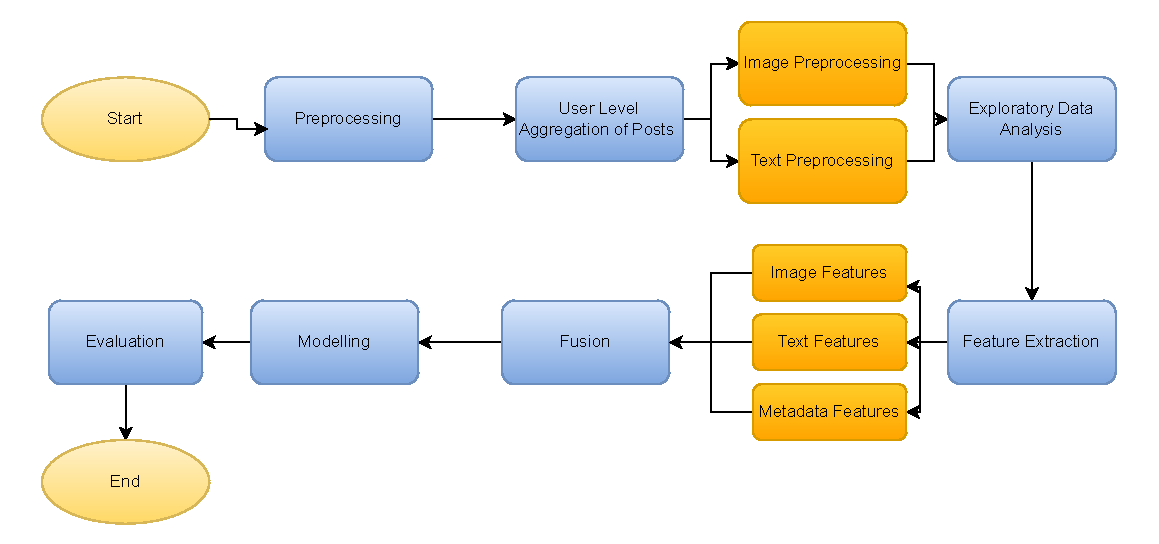
\includegraphics[width=\textwidth]{"figures/Methodology-Flowchart.pdf"}
	\caption{Methodology Flowchart}
	\label{fig:methodology_pipeline}
\end{figure}

\section{Data Source}
\label{sec:data}
This research uses the Instagram subset of the PagkataoKo dataset, a resource specifically created for Filipino APR studies. This dataset fits our study well because it includes user-generated content like posts and images, demographic information, and self-reported Big Five personality scores, which are essential for supervised machine learning. The original Instagram subset has data from 1,380 Filipino users, totaling 195,757 posts. 

We will set specific inclusion criteria to ensure data quality and suitability for a multimodal analysis. The  thresholds that will be based on EDA findings to achieve an optimal balance between data quantity and quality. 

\subsection{Personality Score Transformation to Labels}
In its raw form, the PagkataoKo dataset provides personality scores as continuous numerical values ranging from 1.0 to 5.0 for each of the Big Five traits. Since this study frames personality recognition as a classification task, these continuous scores must be transformed into discrete labels.

To achieve this, a \textbf{median split} will be performed for each of the five personality traits independently. For a given trait (e.g., Openness), users with a score above the median value for that trait will be assigned the 'High' label (e.g., 'High-Openness'). Users with scores at or below the median will be assigned the 'Low' label (e.g., 'Low-Openness'). This process will result in five separate binary labeling schemes, one for each personality dimension, which will serve as the target variables for the classification models.

\subsection{Data Splitting}
For model training and evaluation, the dataset will be divided using a user-level stratified split for model training and evaluation: \textbf{70\%} for training, \textbf{15\%}for validation, and \textbf{15\%} for testing. To ensure that the proportion of 'High' and 'Low' labels for each personality trait is consistent across these sets, the split will be stratified based on the generated personality labels. This helps prevent model bias and ensures that the models are trained and evaluated on representative distributions of each personality class.

\section{Preprocessing}
This stage cleans and organizes the raw data to make it suitable for feature extraction. It is important to normalize multilingual text, manage platform-specific noise, and combine data into a usable format. The main task is \textbf{user-level aggregation}. Here, all posts, images, and metadata for a single user are collected into a single behavioral profile. This method lets the models learn from a user's digital footprint.

\subsection{Image Preprocessing}
All images will go through preprocessing to get them ready for the VGG-19 model. Each image will be resized to 224x224 pixels to fit the model’s required input size. We will also check for corrupted image files. Any posts with unreadable images will be flagged and excluded from the image-based feature extraction process.  

\subsection{Text Preprocessing}
A basic text cleaning method will be used to keep as much of the original content as possible, including multilingual text. The process will involve breaking down the raw caption text into tokens and replacing things like URLs and user mentions with generic tokens (e.g., URL, USER) instead of removing them completely. This way, we keep the context of where a link or mention appeared. All languages will be kept in the text.


\section{Exploratory Data Analysis}
\label{subsec:eda}

Before feature extraction, we will conduct exploratory data analysis (EDA) to understand the key features of the dataset. This analysis will aim to pinpoint demographic trends and content patterns that can guide feature engineering and model interpretation.

The demographic distribution of the final 1,300-user subset, as derived from the PagkataoKo dataset paper, is summarized in Table 4.1. The data shows a user base that is predominantly young (49.3\% aged 18-20) and female (78.0\%). Linguistically, captions are overwhelmingly English-dominant (75.6\%), with a smaller portion being Tagalog-dominant (4.3\%) or exhibiting code-switching (19.4\%).

\begin{table}[h]
	\centering
	\caption{Demographic distribution of Instagram subset (n=1,300)}
	\label{tab:demo}
	\begin{tabular}{lcc}
		\hline
		\textbf{Characteristic} & \textbf{Category} & \textbf{Percentage} \\ \hline
		\textbf{Age} & 18-20 & 49.3\% \\
		& 21-23 & 31.3\% \\
		& 24-26 & 10.7\% \\
		& $\geq$27 & 8.8\% \\ \hline
		\textbf{Sex} & Female & 78.0\% \\
		& Male & 20.0\% \\
		& Intersex/ Declined & 2.0\% \\ \hline
		\textbf{Language} & English-dominant & 75.6\% \\
		& Tagalog-dominant & 4.3\% \\
		& Code-switched & 19.4\% \\ \hline
	\end{tabular}
\end{table}


\section{Feature Extraction}
\label{subsec:features}

This stage focuses on converting the raw text, image, and metadata into quantitative features that machine learning models can process. 

\textbf{Image Features:}
This study will use the \textbf{VGG-19} model, a deep convolutional neural network that has been pre-trained on the ImageNet dataset, to capture high-level visual meanings from the images. For each Instagram image, a \textbf{4,096-dimension feature vector} will be extracted from the second to last fully-connected layer (fc7). This layer is chosen because it captures abstract visual representations like textures and object compositions, which have been shown to be effective in correlating with personality traits. Object detection will use the provided \textbf{Imagga} JSON metadata to quantify the social context of images.  This will allow for the extraction of features such as face counts, which can be linked to traits like Extraversion.  Finally, \textbf{color analysis} will involve generating HSV histograms for each image. K-means clustering, will then be applied to these histograms to identify dominant color palettes.

\textbf{Text Features:}
Instead of using a fixed lexical dictionary, this study will take an open-vocabulary approach to extract textual features. This method lets the models learn directly from the language patterns in the users' captions without being limited to a set dictionary. This approach works well with the mixed nature of the data and is backed by previous research on Filipino APR that found term-frequency features to be effective. Two types of features will be extracted: 

\textbf{TF-IDF Representation}: Term Frequency-Inverse Document Frequency (TF-IDF) will capture the importance of words in a user's collection of captions. The process will create a vocabulary of unigrams and bigrams from the preprocessed text. A TF-IDF vectorizer will then convert each user's combined text into a sparse vector. Each dimension corresponds to a term in the vocabulary, and the value represents the term's weighted importance. This method effectively highlights words that are characteristic of a specific user compared to the overall group.

\textbf{Word Embedding Representation}: Pre-trained FastText word embeddings will capture the semantic meaning of the text. The PagkataoKo dataset paper mentions that these embeddings provide good coverage for the dataset's English and Tagalog words. For each user, the embeddings for all words in their captions will be combined by computing the mean of the vectors. This results in a single, dense vector for each user that represents the overall meaning of their posts. These pre-trained vectors were developed by Grave et al. (2018) and are suitable for this task since they can handle multilingual text.


\textbf{Metadata Features: }
Behavioral signals will be extracted from user account metadata. Features like the Following Ratio (following/followers) and Post Frequency will be calculated and scaled using min-max normalization to show a user's social media activity patterns.

\section{Feature Selection}
Following feature extraction, a feature selection step will be implemented to identify the most relevant predictors for each personality trait. This will be accomplished using the \textbf{Chi-Squared ($\chi^2$) test of independence}, a statistical method well-suited for classification tasks with categorical labels.

The test will be used to evaluate the association between each extracted feature and the binary 'High'/'Low' personality labels. For numerical features, such as TF-IDF scores and metadata values, discretization will be applied to convert them into categorical bins. Features that show a statistically significant association with a personality label (indicated by a low p-value) will be selected for inclusion in the final feature set used for model training. This process helps to reduce model complexity and focus the learning on the most informative signals in the data.

\section{Early Feature Fusion}
\label{subsec:fusion}
This stage employs \textbf{early fusion}(also known as feature-level fusion) features extracted from different sources, including image, text, and metadata, into one unified representation for each user. It aims to make the most of the complementary signals from each data source while keeping dimensionality in check. 

The fusion process starts with standardizing each modality. To lower the high dimensionality of the \texttt{VGG-19} image features and keep the most important information, we will apply \texttt{Principal Component Analysis (PCA)}. After standardization, we will concatenate the feature vectors from all modalities to create a single feature vector for each user. 

\section{Model Training}
\label{subsec:models}

Three distinct classification models will be trained to predict the Big Five personality traits: Logistic Regression, a Support Vector Machine (SVM), and an XGBoost classifier. These models will be implemented using the \texttt{scikit-learn} \citep{pedregosa2011} and \texttt{XGBoost} \citep{chen2016}  Python libraries.

A logistic regression (LR) model will be trained as a strong and interpretable baseline. Its performance will provide a benchmark to compare against the more complex models, making it easier to measure improvements.  

A Support Vector Machine (SVM) will be trained, and its kernel function (e.g., Radial Basis Function (RBF), linear, polynomial) and regularization parameters \texttt{(C, gamma)} will be optimized through a comprehensive grid search to find the best setup for the data.

Lastly, we will also train an XGBoost classifier. This gradient-boosting algorithm effectively handles different types of features and includes a built-in way to assess the importance of those features.

\section{Model Analysis}
\label{subsec:analysis}
A detailed review will be done to assess how well the trained models perform. The main metrics for evaluation will be the \texttt{Macro-F1 score} and the \texttt{Area Under the Receiver Operating Characteristic Curve (AUC-ROC)}. We choose the Macro F1 score because it works well for datasets with uneven class distributions. The AUC-ROC will help us evaluate the model's ability to rank and differentiate between classes. 

We will use \texttt{SHAP (SHapley Additive exPlanations}) to understand how the models make decisions. SHAP helps us measure how much each feature contributes to the model's predictions. This will create plots showing global feature importance, giving a clear ranking of the most impactful visual, textual, and metadata clues for each personality trait. 

Lastly, we will perform \texttt{ablation studies} to systematically compare the performance of the complete multimodal models with unimodal models, such as text-only and image-only. This will help us identify the effect of each modality on performance and see if combining image and text features significantly improves personality prediction accuracy.
